%% Encoding: ISO8859-1 %%

\section{Hauptaussagen}
\frame{
\frametitle{Hauptaussagen}
\begin{itemize}
    \item Signale als Tokens die sich frei auf Kabeln bewegen 
    \item Fluktuation (brownsche Bewegung) der Token als treibende Kraft f�r Berechnungen
    \item T-Element als Grundbaustein 
    \item nicht polare Variante erm�glicht einfacheres Design
\end{itemize}
}
\section{T-Element}
\frame{
\frametitle{T-Element}
\begin{columns}[T]
    \begin{column}[T]{5cm}
            \begin{figure}
                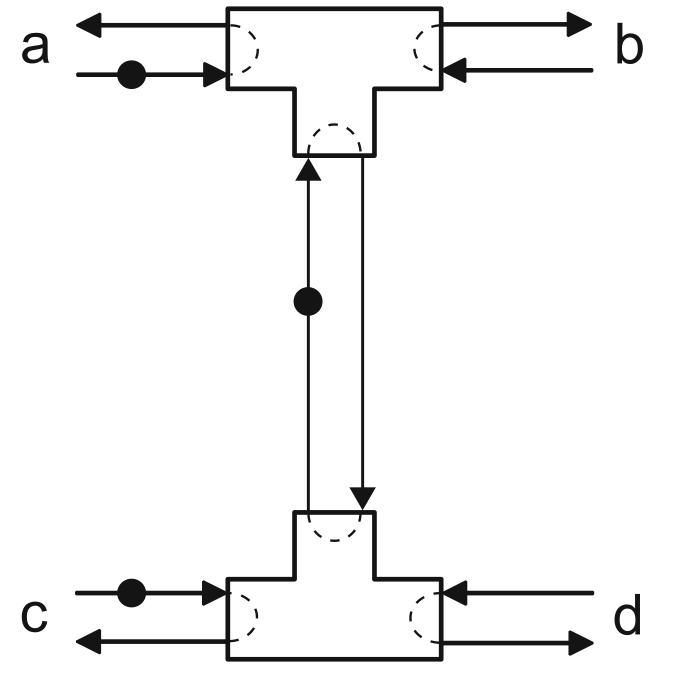
\includegraphics[height=5cm]{bilder/polarElemente.png} 
                \captionsetup{labelformat=empty}
                \caption{polare T-Elemente}
            \end{figure}
    \end{column}
    \begin{column}[T]{5cm}
        \begin{figure}
                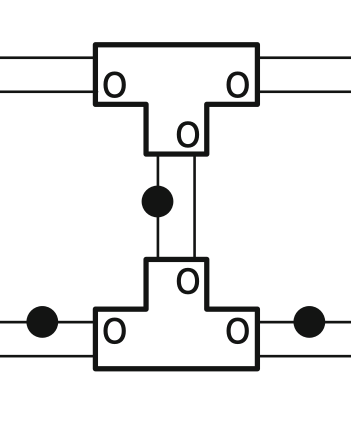
\includegraphics[height=5cm]{bilder/nonPolarElemente.png} 
                \captionsetup{labelformat=empty}
                \caption{nicht polare T-Elemente}
            \end{figure}
    \end{column}
\end{columns}
}


